%!TEX root = Slic3r-Manual.tex

Il ya deux façons d'organiser les paramètres de configuration: exporter et importer les paramètres de configuration, et des profils. Le premier est disponible en mode simple et expert, alors que les profils sont disponibles uniquement en mode expert.

\section{Exporting and Importing Configuration} % (fold)
\label{sub:exporting_and_importing_configuration}
\index{configuration!export}
\index{configuration!import}

L'ensemble actuel d'options de configuration peut être tout simplement exporté via le menu File (Fichier)  \texttt{Export Config}. Cela permet se sauvegarder toutes les valeurs dans un fichier texte avec l'extention \texttt{.ini} .  Les fichiers précédemment enregistrés peuvent être chargés avec le menu File (fichier) \texttt{Load Config} (charger la configuration).

Cela donne un des moyens rudimentaires pour stocker des paramètres de configuration pour les différents besoins. Par exemple, un ensemble avec des vitesses d'impression légèrement plus rapides, ou un motif de remplissage différent. Cependant, cette façon d'organiser les choses va vite devenir frustrante, car chaque changement mineur d'un paramètre pourrait être à dupliqué dans de nombreuses configurations. Pour cette raison, les profils sont de façon plus appropriée de gérer plusieurs configurations.

Cette méthode permet également le transfert de configurations entre machines, ou le stockage à distance.

% section exporting_and_importing_configuration (end)


\section{Profiles} % (fold)
\label{sec:profiles}
\index{profiles}
\index{profils}

Après quelques impressions, il deviendra évident qu'il est utile d'avoir un ensemble d'options de configuration à choisir, et que certains paramètres changent plus souvent que d'autres. En mode expert, des profils peuvent être créés pour les paramètres d'impression, de Filament et d'imprimante, dans l'espoir que les paramètres d'imprimante changent peu souvent, de filaments rarement, cependant les paramètres d'impression peuvent être modifiés pour chaque modèle. Ces différents profils peuvent être mélangés et combinés à volonté, et peuvent être sélectionnés dans leurs onglets respectifs, ou directement à partir de la surface de travail.

\subsection{Creating Profiles} % (fold)
\label{sub:creating_profiles}
\index{profiles!create}
\index{profils!création}

Ouvrez l'onglet souhaité et modifiez les paramètres si nécessaire. Une fois satisfait, cliquez sur l'icône de sauvegarde vers la gauche au-dessus des titres de réglage, et donner un nom approprié à l'invite.

\begin{figure}[H]
\centering
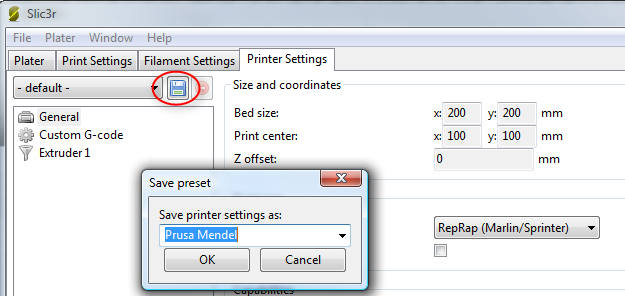
\includegraphics[keepaspectratio=true,width=1\textwidth]{organising/creating_a_profile.png}
\caption{Sauver un profil.}
\label{fig:creating_a_profile}
\end{figure}

\index{profiles!delete}
\index{profils!effacer}
Les profils peuvent être supprimés, en choisissant le profil à supprimer et en cliquant sur le bouton rouge supprimer à côté du bouton Enregistrer.

\begin{figure}[H]
\centering
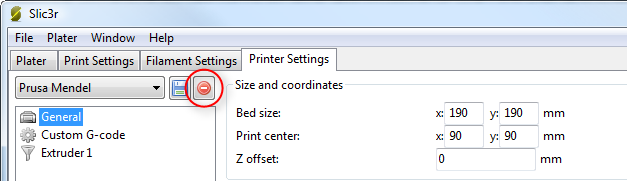
\includegraphics[keepaspectratio=true,width=1\textwidth]{organising/deleting_a_profile.png}
\caption{Effacer un profil.}
\label{fig:deleting_a_profile}
\end{figure}

% subsection creating_profiles (end)


% section profiles (end)